% This example is meant to be compiled with lualatex
\PassOptionsToPackage{unicode}{hyperref}
\documentclass[aspectratio=1610, 9pt]{beamer}


\usetheme[
  % ShowTotalFrames,               % show total number of frames in the footline
  ProgressBar,                     % show progressbar
  % ProgressBarStart=1,            % start progressbar at page 1
]{code}


\input{headers/header.tex}


% Put settings here, like
\unimathsetup{
  math-style=ISO,
  bold-style=ISO,
  nabla=upright,
  partial=upright,
  mathrm=sym,
}

\title{Resource-Aware \\Deep Learning}
\subtitle{Tracking Energy Consumption in Scientific \\AI Applications}

\author[K. Schmitz \& A.~Knierim]{Kevin Schmitz\hspace{2cm}Anno Knierim}
\contact{{\large{\faGithub}}\:kevin2\hspace{3.2cm}{\large{\faGithub}}\:aknierim}
\date{March 15, 2026}


\begin{document}

\maketitle

\begin{frame}{Why Resource Awareness Matters}
  \begin{columns}
    \begin{column}{0.55\textwidth}
      \begin{itemize}
        \setlength{\itemsep}{1.5em}
        \item Growing computational demands of AI in physics
        \item Environmental impact: CO$_2$ footprint of training and inference
        \item Compute costs and computing cluster resource allocation
        \item Tracking resources as part of scientific documentation and reproducibility
      \end{itemize}
    \end{column}
    \begin{column}{0.45\textwidth}
      \centering
      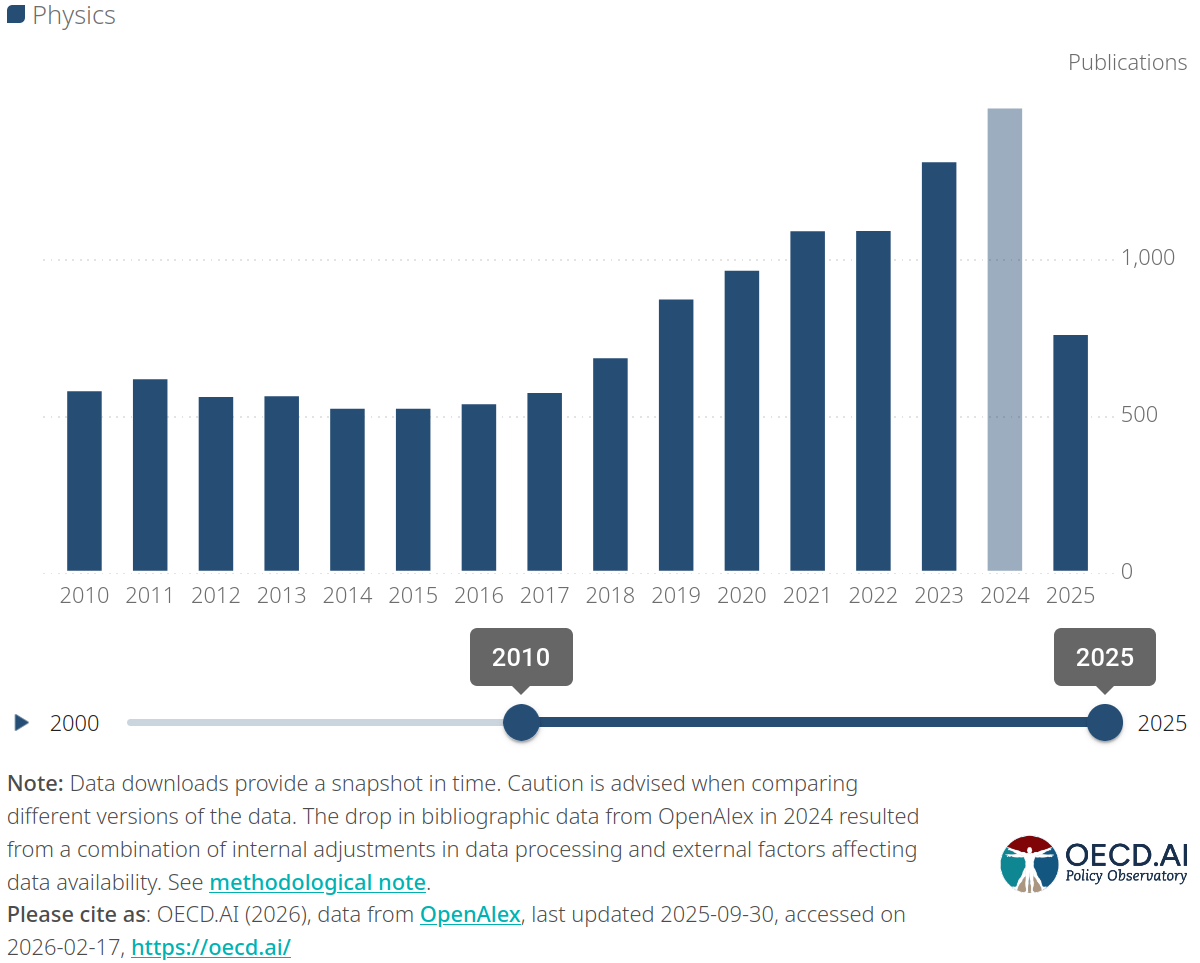
\includegraphics[width=\textwidth]{images/AI_physics_publications.png}
      \Tiny\texttt{[https://oecd.ai/en/data?selectedArea=ai-research]}
    \end{column}
  \end{columns}
\end{frame}

\begin{frame}{AI Applications in Physics}
  \begin{columns}
    \begin{column}{0.5\textwidth}
      \begin{itemize}
        \setlength{\itemsep}{1.5em}
        \item Source identification in astronomy
        \item Particle track reconstruction in high-energy physics
      \end{itemize}
    \end{column}
    \begin{column}{0.5\textwidth}
      \begin{itemize}
        \setlength{\itemsep}{1.5em}
        \item Refinement in medical imaging
        \item Large language models for many applications
      \end{itemize}
    \end{column}
  \end{columns}

  \vspace{0.5cm}
  \centering
  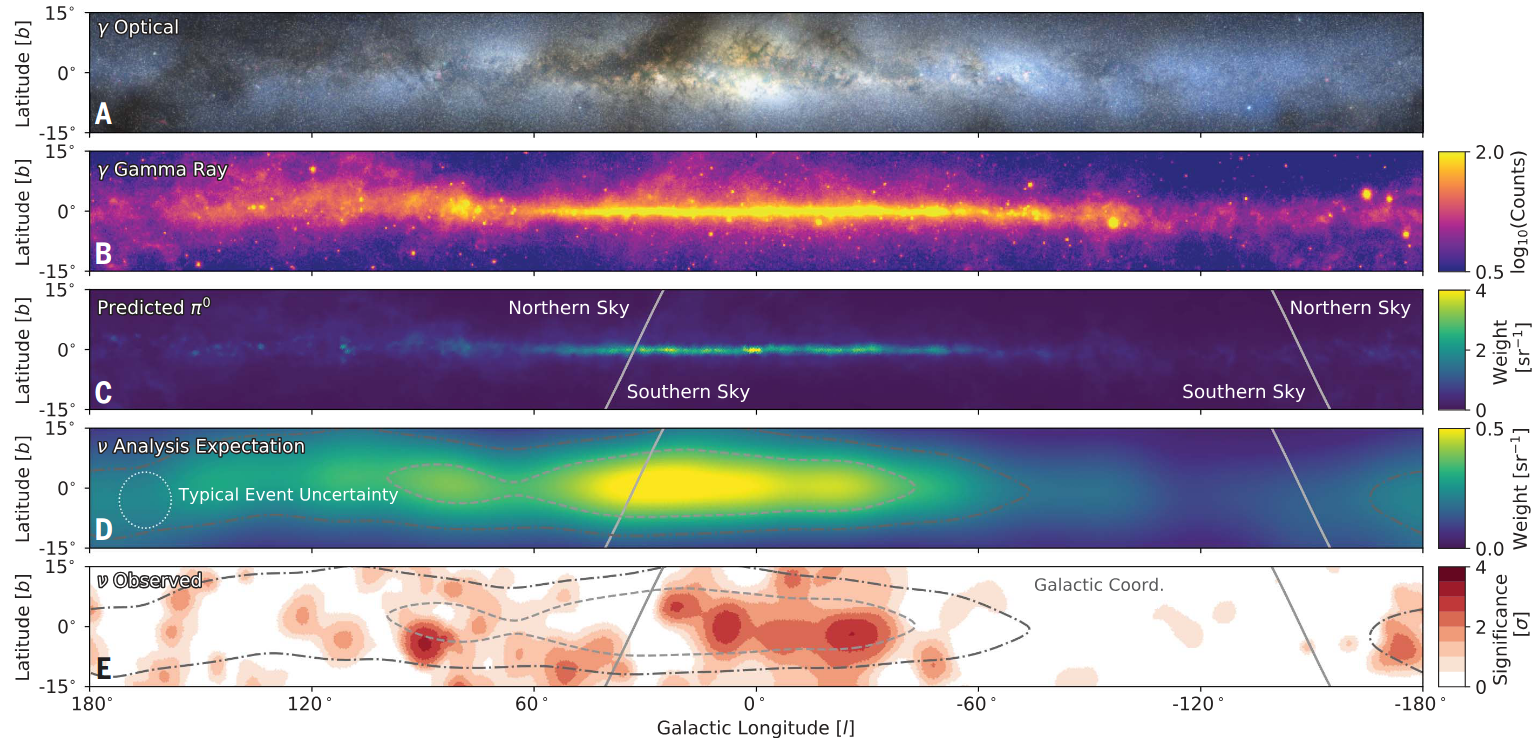
\includegraphics[width=0.75\textwidth]{images/neutrinos_milkyway.png}\\
  \Tiny\texttt{[IceCube Collaboration, Science 2023]}
\end{frame}

\begin{frame}{DFG Sustainability Guidelines}
  \centering
  
\includegraphics[width=.8\textwidth]{images/dfg_sustainability.png}
  \Tiny\texttt{[https://www.dfg.de/en/basics-topics/developments-within-the-research-system/sustainability-guide-for-research-processes]}
\end{frame}

\begin{frame}{AI Workflows in Physics}
  \centering
  \begin{tikzpicture}[
    every node/.style={align=center},
    arrow/.style={
        ->,
        -{Stealth[length=8pt]},
        thick,
        shorten >=4pt,
        shorten <=4pt
    },
    scale=0.7,
]




% ---- Simulations & Data Processing (left side) ----

\def\cx{-8.5}
\def\cy{0.45}
\def\cs{0.75}
\def\ov{0.4}
\def\nr{0.1}

\coordinate (A) at (\cx,     \cy+\ov*2);
\coordinate (B) at (\cx-\cs, \cy+\ov);
\coordinate (C) at (\cx,     \cy);
\coordinate (D) at (\cx+\cs, \cy+\ov);
\coordinate (E) at (\cx-\cs, \cy-\cs+\ov);
\coordinate (F) at (\cx,     \cy-\cs);
\coordinate (G) at (\cx+\cs, \cy-\cs+\ov);

\draw[thick] (A) -- (B) -- (C) -- (D) -- cycle;
\draw[thick] (B) -- (C) -- (F) -- (E) -- cycle;
\draw[thick] (D) -- (C) -- (F) -- (G) -- cycle;

\foreach \pt in {A, B, C, D, E, F, G}
    \fill (\pt) circle (\nr);

\node[font=\itshape] at (\cx, -1.1) {Simulations \&\\Data Processing};
\draw[arrow, thick] (\cx+1.6, 0.0) -- (-2.9, 0.0);

% ---- Circle diagram ----
% Three arcs that together form the complete circle, each with an arrow.
% They meet exactly: 150->30, 30->-90, -90->-210 (=-210+360=150)

\draw[thick, ->, -{Stealth[length=8pt]}]
    ([shift={(150:2.8cm)}]0,0)
    arc[start angle=150, end angle=30, radius=2.8cm];

\draw[thick, ->, -{Stealth[length=8pt]}]
    ([shift={(30:2.8cm)}]0,0)
    arc[start angle=30, end angle=-90, radius=2.8cm];

\draw[thick, ->, -{Stealth[length=8pt]}]
    ([shift={(-90:2.8cm)}]0,0)
    arc[start angle=-90, end angle=-210, radius=2.8cm];

% Flask
\draw[thick]
    (-0.2,  0.85) -- (-0.2,  0.45)
    .. controls (-0.2,  0.2 ) and (-0.52,-0.07) .. (-0.52,-0.33)
    .. controls (-0.52,-0.52) and ( 0.52,-0.52) .. ( 0.52,-0.33)
    .. controls ( 0.52,-0.07) and ( 0.2,  0.2 ) .. ( 0.2,  0.45)
    -- ( 0.2,  0.85) -- cycle;
\draw[thick] (-0.23, 0.85) -- (0.23, 0.85);

\node[font=\large\itshape] at (0, -1.0) {Experiments};

% Outer labels at arc midpoints
\node[font=\itshape] at (90:4.0cm)   {model\\development};
\node[font=\itshape] at (-30:4.2cm)  {uncertainty\\quantification};
\node[font=\itshape] at (-150:4.0cm) {parameter\\tuning};

% ---- Production Inference (right side) ----

\draw[thick]
    (7.3,  -0.35) --
    (7.3,   0.9)  --
    (7.65,  0.9)  --
    (7.65,  0.1)  --
    (8.05,  0.5)  --
    (8.05,  0.1)  --
    (8.45,  0.5)  --
    (8.45,  0.1)  --
    (8.85,  0.5)  --
    (8.85, -0.35) --
    cycle;

\draw[thick] (7.48, 1.1)  circle (0.11);
\draw[thick] (7.60, 1.35) circle (0.14);
\draw[thick] (7.43, 1.60) circle (0.18);

\node[font=\itshape] at (8.075, -1.1) {Production\\Inference};
\draw[arrow, thick] (2.9, 0.0) -- (7.0, 0.0);

\end{tikzpicture}
\end{frame}

\begin{frame}{ML tracking/monitoring in scientific workflows}
  \begin{columns}
    \begin{column}{0.55\textwidth}
      \begin{itemize}
        \setlength{\itemsep}{1.5em}
        \item Need for reproducibility in scientific research
        \item Documentation requirements for publications
        \item Integration with existing workflows
        \item MLflow\footnote{\url{https://mlflow.org/}} / Weights \& Biases\footnote{\url{https://wandb.ai/}} / Comet\footnote{\url{https://www.comet.com/site/}}
      \end{itemize}
    \vspace*{1cm}
    \end{column}
    \begin{column}{0.45\textwidth}
      \centering
      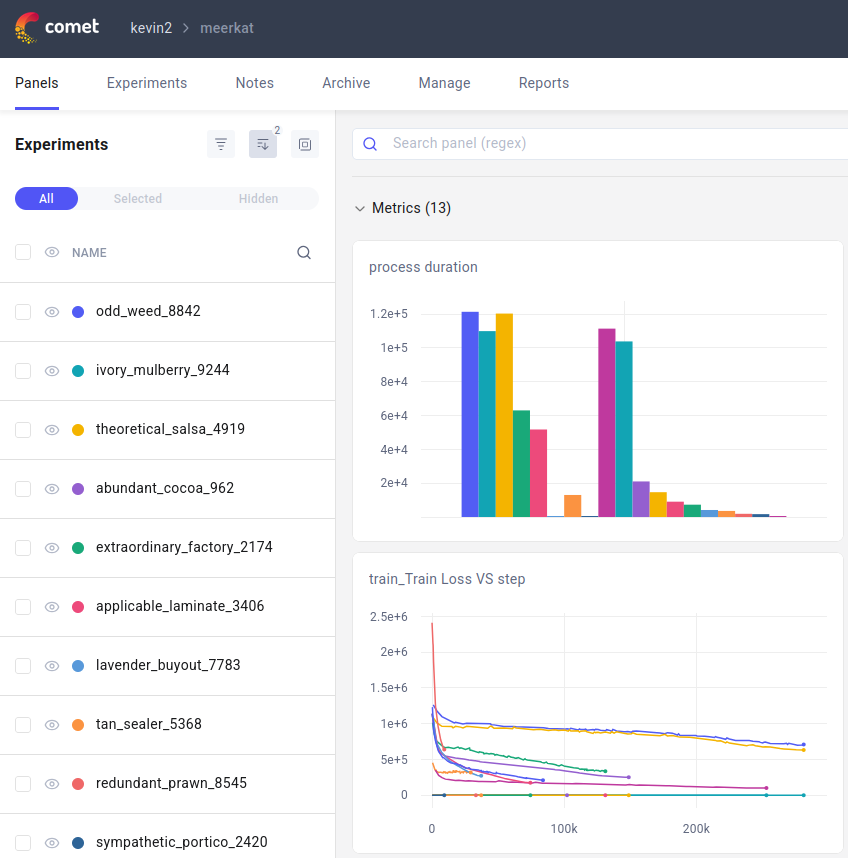
\includegraphics[width=\textwidth]{images/comet.png}
    \end{column}
  \end{columns}
\end{frame}

\begin{frame}{Measuring Resource Consumption}
  \begin{columns}
    \begin{column}{0.55\textwidth}
      \begin{itemize}
        \setlength{\itemsep}{1.5em}
        \item Energy consumption (kWh, CO$_2$ equivalent)
        \item GPU/CPU utilization
        \item Memory usage
        \item Training times
        \item Inference times
      \end{itemize}
    \end{column}
    \begin{column}{0.45\textwidth}
      % \centering
      % 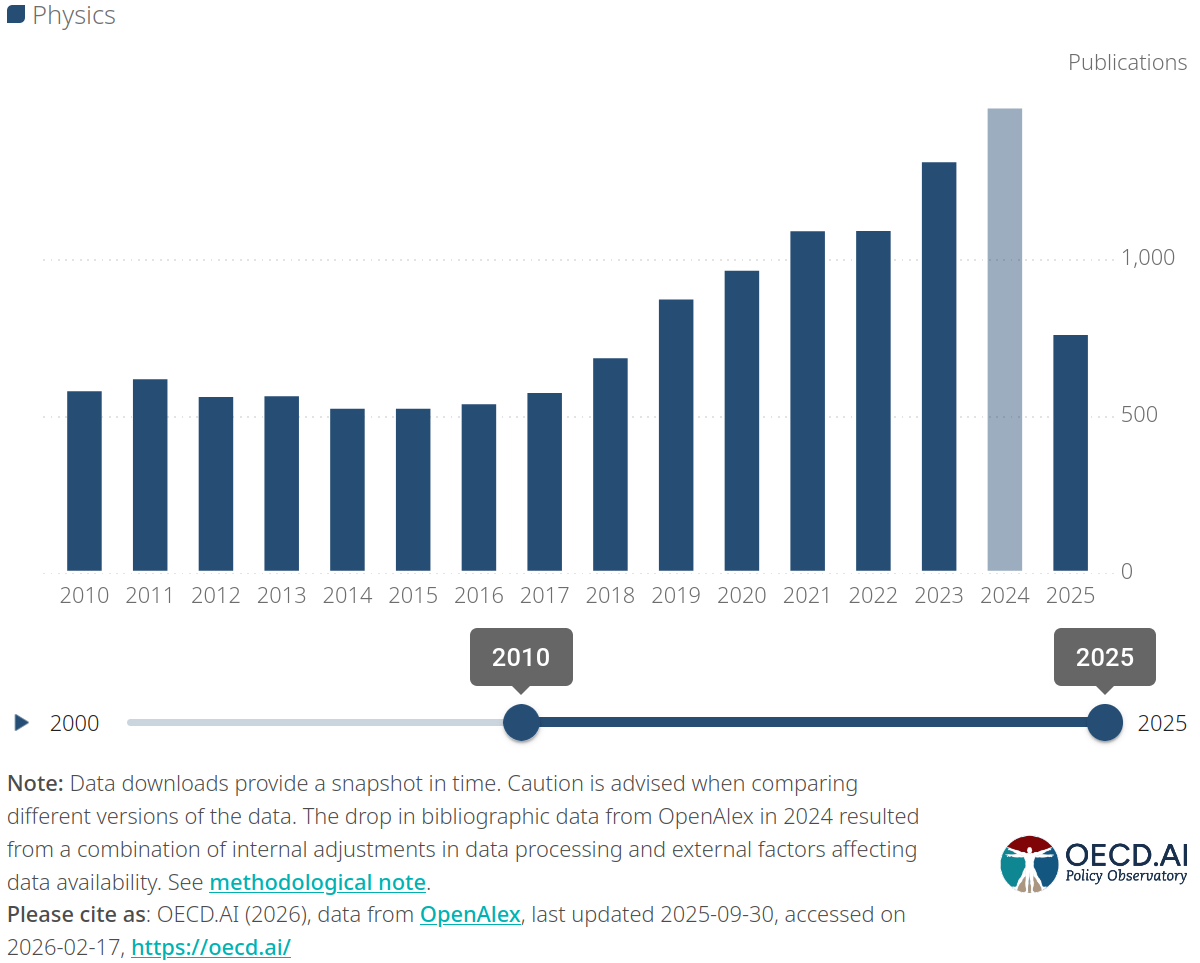
\includegraphics[width=\textwidth]{images/AI_physics_publications.png}
    \end{column}
  \end{columns}
\end{frame}

\begin{frame}{Typical Resource Profile in Physics AI Applications}
  \begin{columns}
    \begin{column}{0.55\textwidth}

    \begin{table}
      \centering
      \begin{tabular}{lcc}
        \toprule
        \textbf{Workflow Stage} & \textbf{Time} & \textbf{Energy} \\
        \midrule
        \textbf{Data Creation:} & & \\
        Simulation Generation & X hours & Y kWh \\
        Data Preprocessing & X hours & Y kWh \\
        \midrule
        \textbf{Development Cycle:} & & \\
        Model Selection & X hours & Y kWh \\
        Hyperparameter Tuning & X hours & Y kWh \\
        Loss Selection & X hours & Y kWh \\
        \midrule
        \textbf{Production:} & & \\
        Inference Run & X hours & Y kWh \\
        \midrule
        \textbf{Development Total} & XX hours & YY kWh \\
        \bottomrule
      \end{tabular}
    \end{table}
    \end{column}
    \begin{column}{0.45\textwidth}
      % \centering
      % 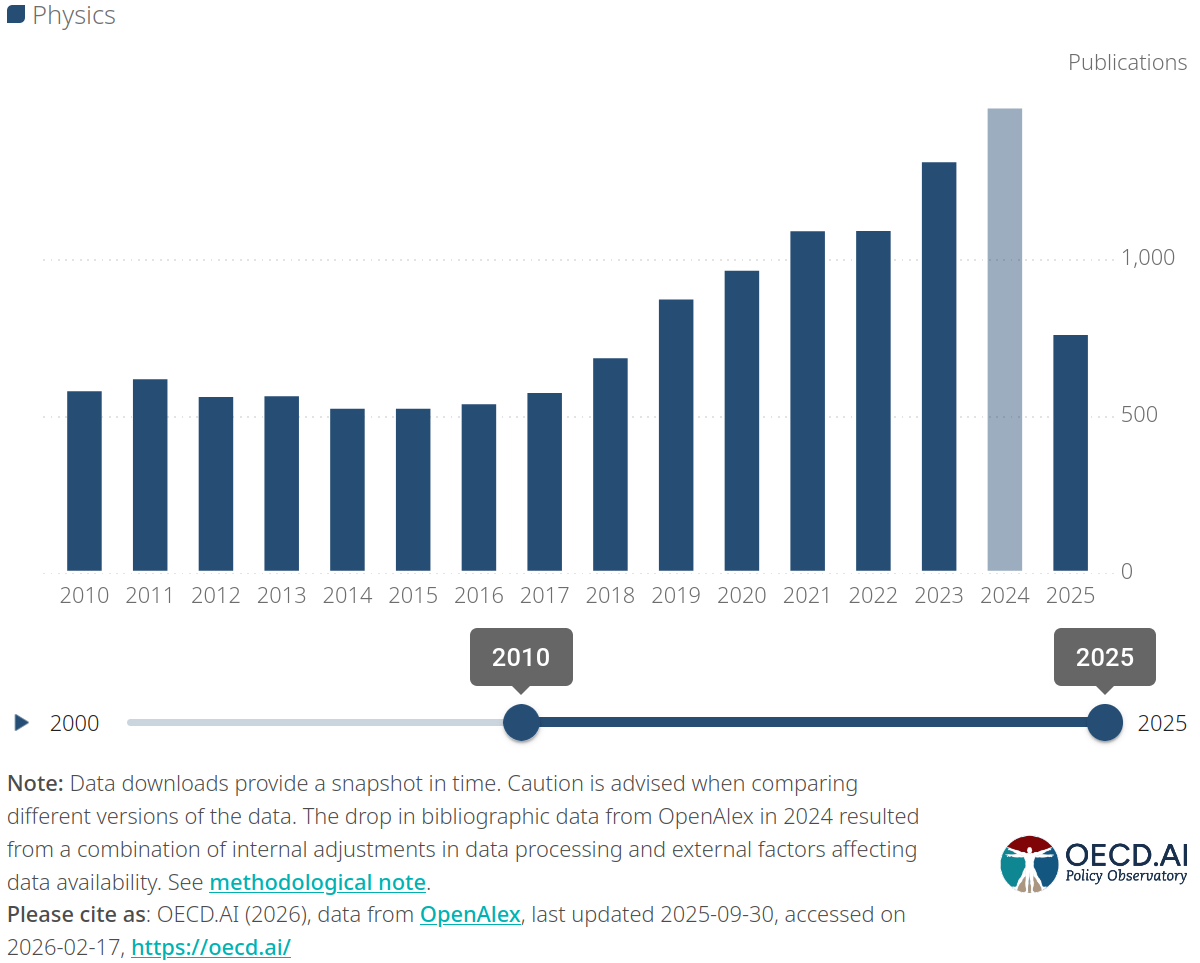
\includegraphics[width=\textwidth]{images/AI_physics_publications.png}
    \end{column}
  \end{columns}
\end{frame}


\begin{frame}{Available Tracking Methods}

  \centering
  {\bf{Static Estimation} \hspace{2cm} {Dynamic Estimation} \hspace{2cm} {External Measurement}}\\
  \vspace*{1cm}
  \centering
  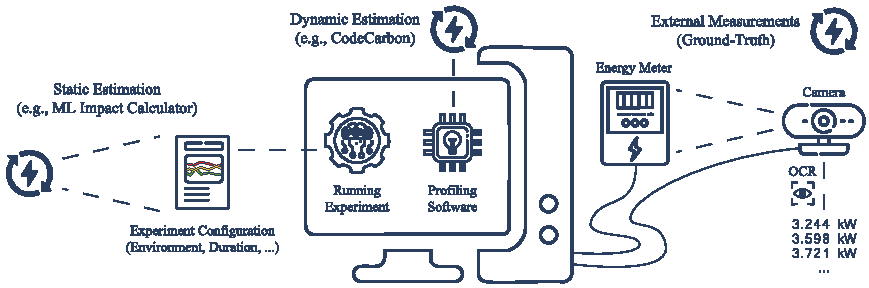
\includegraphics[width=\textwidth]{images/fig2.pdf}
  \Tiny\texttt{[arXiv:2509.22092]}

\end{frame}

\begin{frame}{Static Estimation}
  
  \begin{columns}
    \begin{column}{0.55\textwidth}
      \begin{itemize}
        \setlength{\itemsep}{1.5em}
        \item Statistical estimation
        \item Based on configuration and environment
        \item CO$_2$ Equiv. = Power ~\cdot~ Time ~\cdot~ CO$_2$ Efficiency
        \item ML Impact Calculator\footnote{\url{https://www.climatechange.ai/papers/neurips2019/22}}
        \item No flexible adjustments
      \end{itemize}
      \vspace*{1cm}
    \end{column}
    \begin{column}{0.45\textwidth}
      \centering
      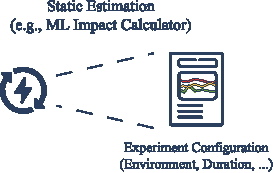
\includegraphics[height=2.5cm]{images/static_est.pdf}\\
      \Tiny\texttt{[arXiv:2509.22092]}
    \end{column}
  \end{columns}
\end{frame}


\begin{frame}{Dynamic Estimation}
  
  \begin{columns}
    \begin{column}{0.55\textwidth}
      \begin{itemize}
        \setlength{\itemsep}{1.5em}
        \item Profiling dynamic resource demand
        \item Power x Running Time
        \item Profiling software: experiment-impact-tracker\footnote{\url{https://arxiv.org/abs/2002.05651}} / CodeCarbon\footnote{\url{https://codecarbon.io/}}
        \item Power Draw per short time interval
        \item Misses power supply and cooling
      \end{itemize}
      \vspace*{1cm}
    \end{column}
    \begin{column}{0.45\textwidth}
      \centering
      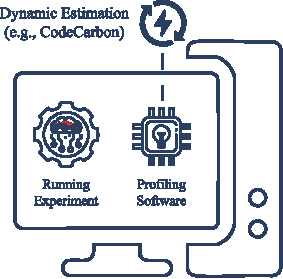
\includegraphics[height=4cm]{images/dynamic_est.pdf}\\
      \Tiny\texttt{[arXiv:2509.22092]}
    \end{column}
  \end{columns}
\end{frame}

\begin{frame}{External Measurements}
  
  \begin{columns}
    \begin{column}{0.55\textwidth}
      \begin{itemize}
        \setlength{\itemsep}{1.5em}
        \item Ground-truth energy consumption
        \item Capture impact of all components\\
        \rightarrow external measurement
        \item Energy meter + camera + computer vision code
        \item Energy meter between power supply and hardware
        \item But: additional hardware and implementation effort
      \end{itemize}
      \vspace*{1cm}
    \end{column}
    \begin{column}{0.45\textwidth}
      \centering
      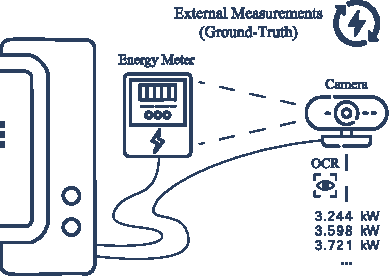
\includegraphics[height=4cm]{images/external_est.pdf}\\
      \Tiny\texttt{[arXiv:2509.22092]}
    \end{column}
  \end{columns}
\end{frame}

\begin{frame}{Combined Tracking}

  \centering
  {\bf{Static Estimation} \hspace{2cm} {Dynamic Estimation} \hspace{2cm} {External Measurement}}\\
  \vspace*{1cm}
  \centering
  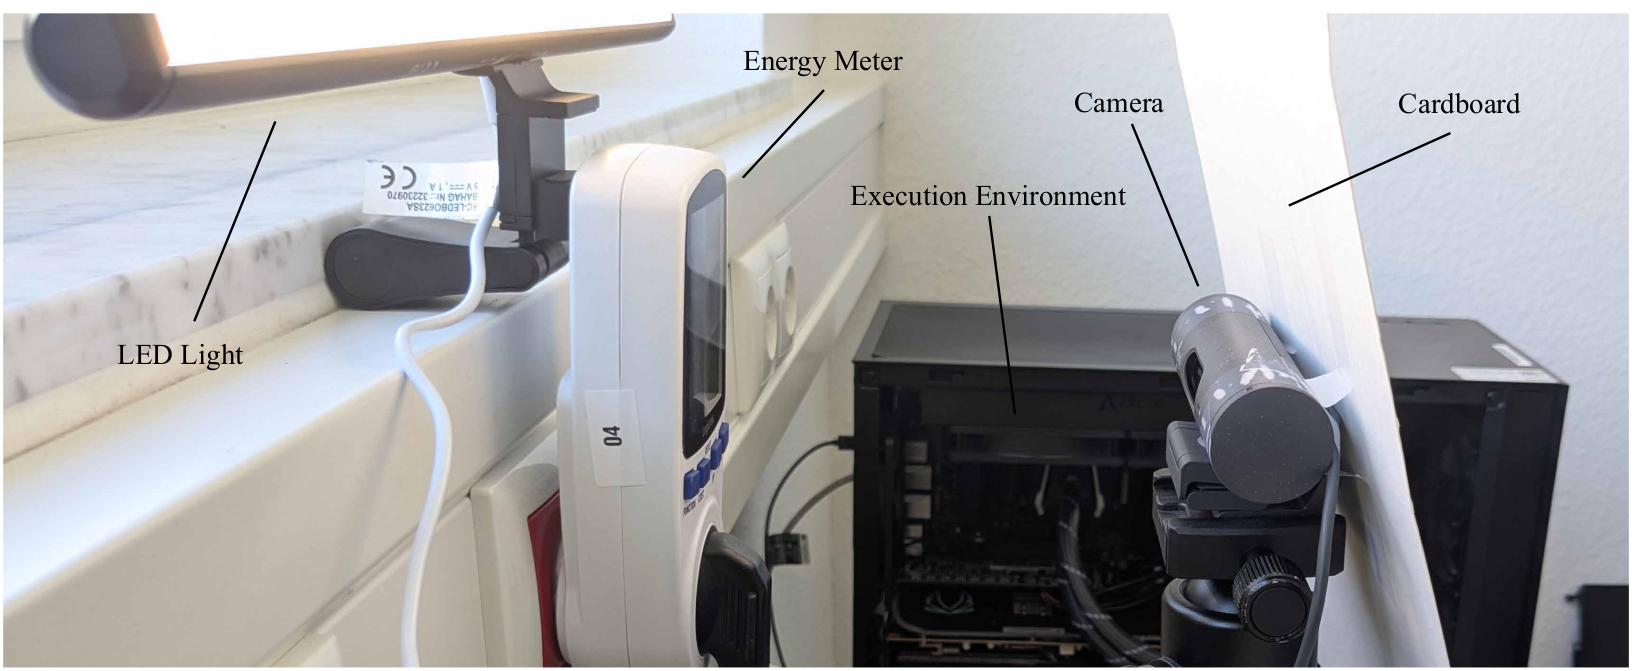
\includegraphics[width=\textwidth]{images/experimental_setup.png}
  \Tiny\texttt{[arXiv:2509.22092]}

\end{frame}


\begin{frame}{LAMARR Energy Tracker (LET)}

  \centering
  {\bf{Static Estimation} \hspace{2cm} {Dynamic Estimation} \hspace{2cm} {External Measurement}}\\
  \vspace*{1cm}
  \centering
  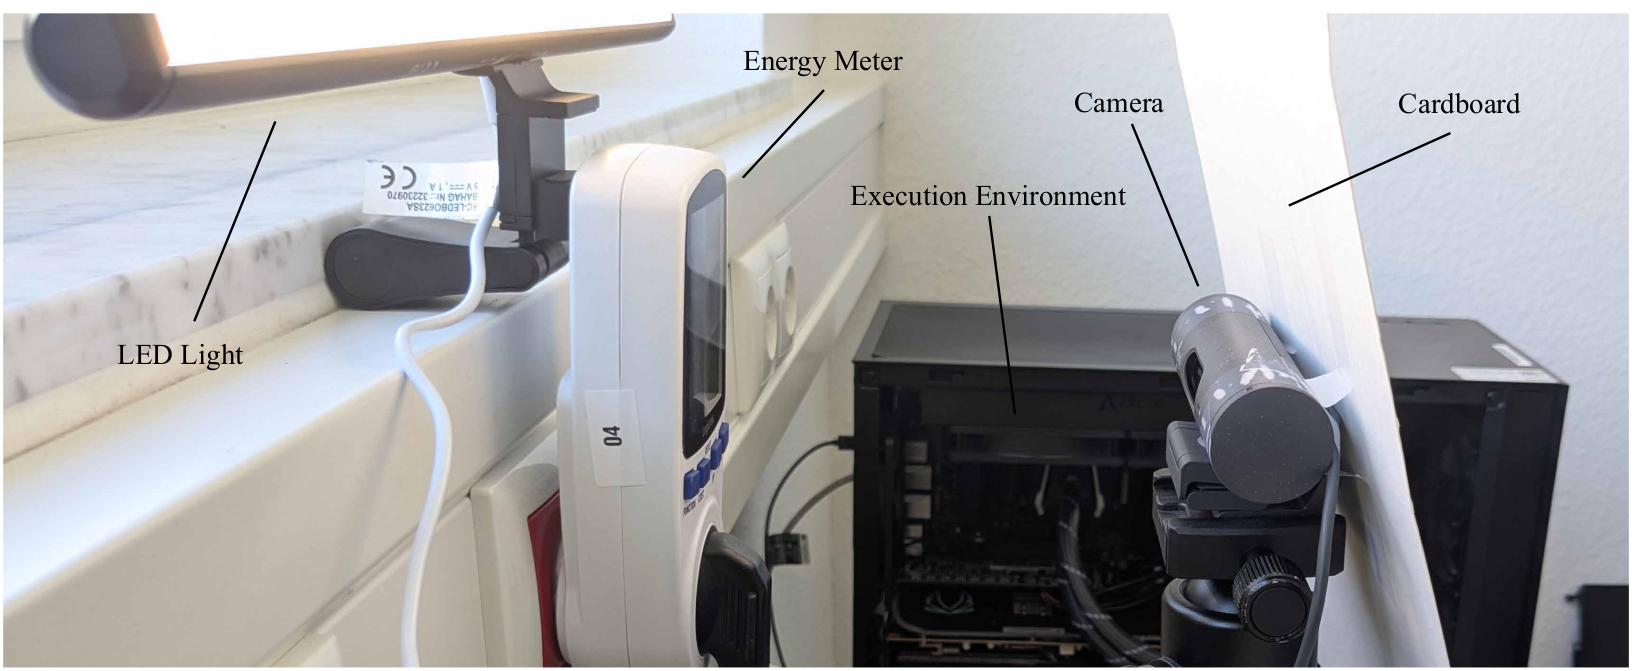
\includegraphics[width=\textwidth]{images/experimental_setup.png}
  \Tiny\texttt{[arXiv:2509.22092]}

\end{frame}

\begin{frame}{STREP}

  \centering
  {\bf{Static Estimation} \hspace{2cm} {Dynamic Estimation} \hspace{2cm} {External Measurement}}\\
  \vspace*{1cm}
  \centering
  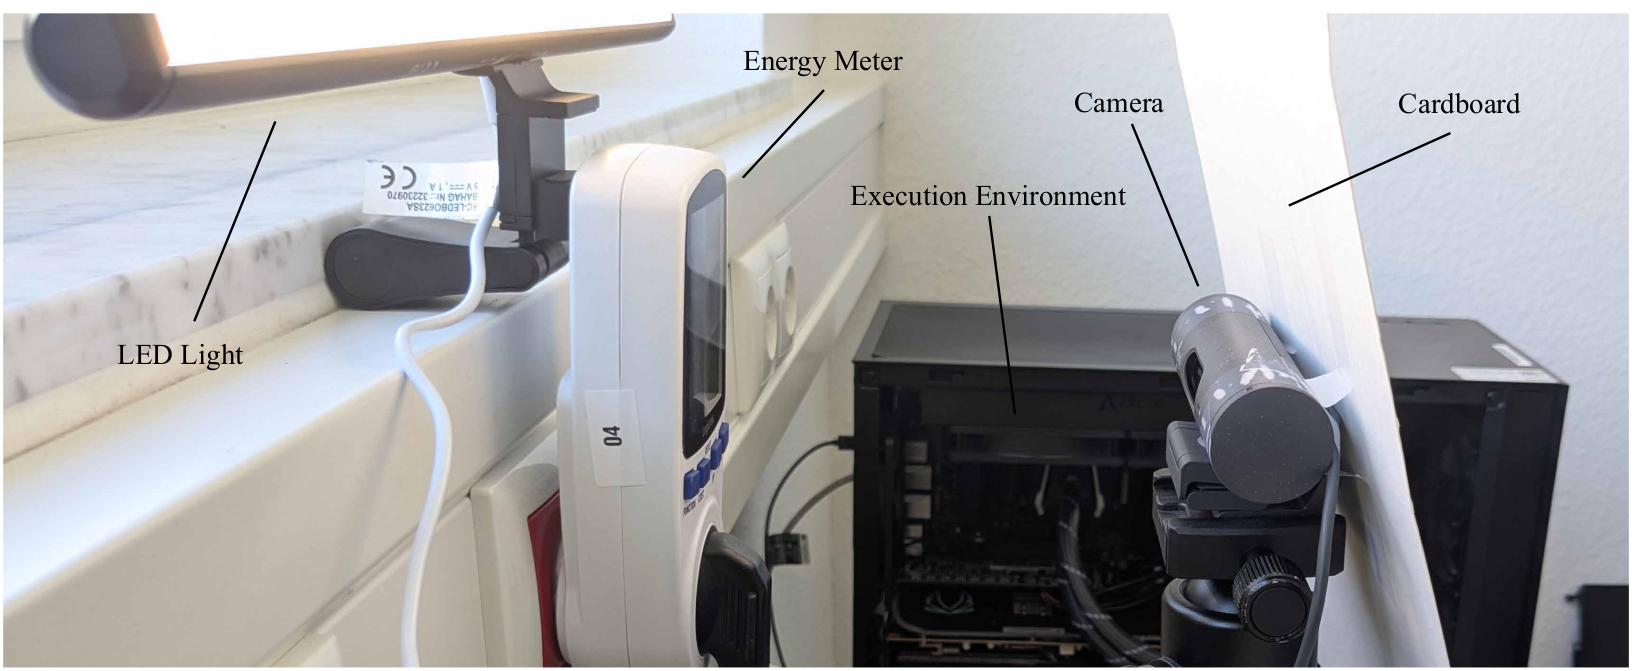
\includegraphics[width=\textwidth]{images/experimental_setup.png}
  \Tiny\texttt{[arXiv:2509.22092]}

\end{frame}

\begin{frame}{Final Advices}

  \centering
  {\bf{Static Estimation} \hspace{2cm} {Dynamic Estimation} \hspace{2cm} {External Measurement}}\\
  \vspace*{1cm}
  \centering
  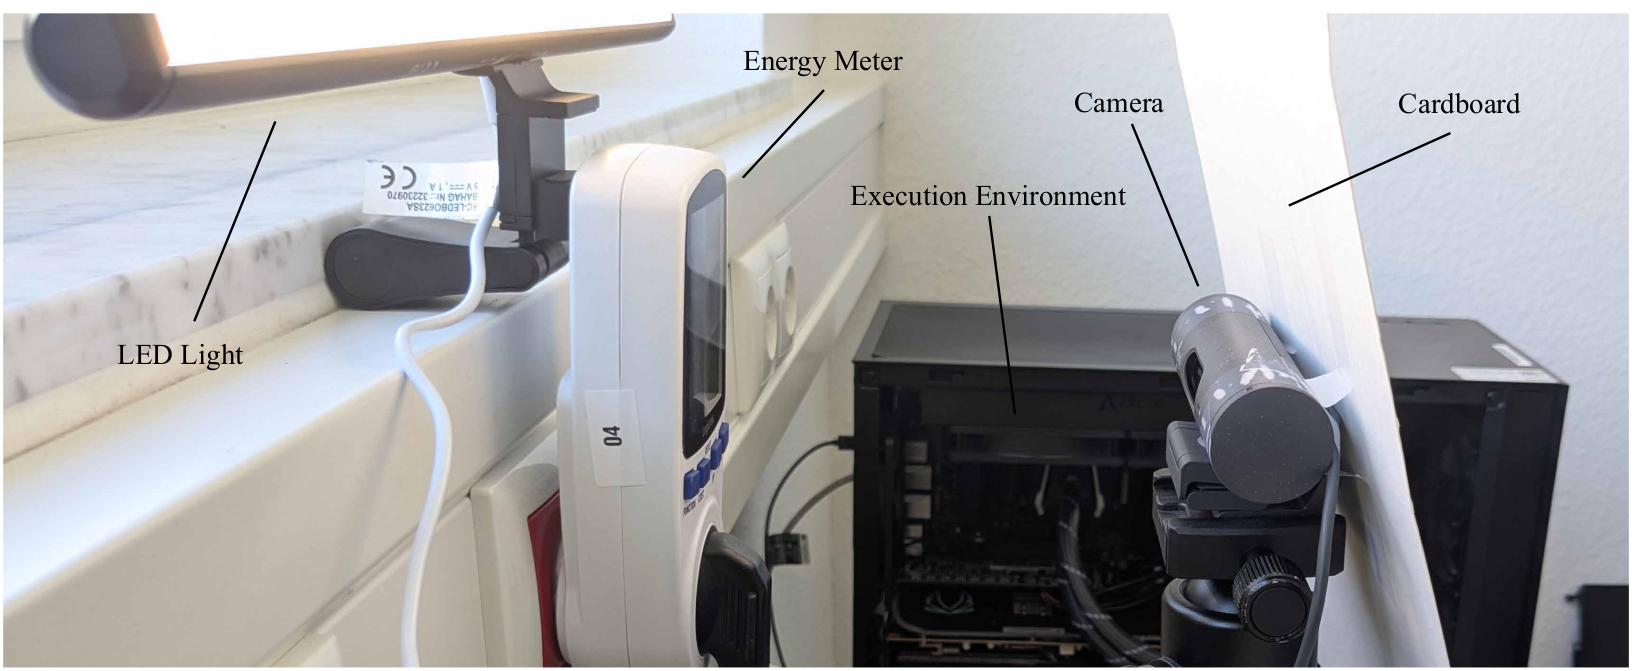
\includegraphics[width=\textwidth]{images/experimental_setup.png}
  \Tiny\texttt{[arXiv:2509.22092]}

\end{frame}

\end{document}
